
\documentclass[a4paper,11pt]{report}
\usepackage[utf8]{inputenc}
\usepackage[T1]{fontenc}
\usepackage{lmodern}
\usepackage[ngerman]{babel}
\usepackage[margin=20mm, left=20mm, right=10mm, headheight=15pt, includeheadfoot]{geometry}
\usepackage{fancyhdr}
\usepackage{opensans}
\usepackage{titlesec}
\usepackage{tocloft}
\usepackage{titling}
\usepackage{hyperref}
\usepackage{graphicx}
\usepackage{enumerate}
\usepackage{float}
\usepackage{caption}
\usepackage{listings}
\usepackage{wrapfig}
\usepackage{minted}
\usepackage{subcaption}
\usemintedstyle{vs}

% Set default font to OpenSans
\renewcommand*\familydefault{\sfdefault}

% Page style for cover page
\fancypagestyle{cover}{
    \fancyhf{}
    \renewcommand{\headrulewidth}{0pt}
    \renewcommand{\footrulewidth}{0pt}
}

% Page style for main content
\fancypagestyle{main}{
    \fancyhf{}
    \fancyhead[L]{\theauthor}
    \fancyhead[R]{\subject}
    \fancyfoot[C]{\thepage}
    \renewcommand{\headrulewidth}{0.4pt}
    \renewcommand{\footrulewidth}{0pt}
}

\titleformat{\chapter}[block]
  {\normalfont\Large\bfseries} % change \Large to \large or any other size that fits
  {\thechapter}
  {1em}
  {}

  \titlespacing*{\chapter}{0pt}{*4}{*2.5}

% Graphics path
\graphicspath{ {./images/} }

% Cover page
\newcommand{\coverpage}{
    \thispagestyle{cover}
    \pagenumbering{roman} % Start Roman numbering for the cover page
    \begin{center}
        {
\includegraphics[height=3cm]{fh-logo}}\\[1cm]
        {\LARGE \thetitle}\\[0.5cm]
        {\large \theauthor}\\
    \end{center}
    \tableofcontents
    \clearpage
}

% Author and subject
\author{Felix Hillebrand}
\newcommand{\subject}{AMS4UE}

% Main document
\begin{document}
    % Color definitions
    \definecolor{LightGray}{gray}{0.9}
    \definecolor{DarkGray}{gray}{0.3}

    \title{AMS~-~UE}
    \coverpage

    \clearpage
    \pagestyle{main}
    \pagenumbering{arabic} % Start Arabic numbering for main content

% ------------------------------------------
% --        Main document starting        --
% ------------------------------------------

    \chapter{Spannbaum Prim}
    \label{ch:spbprim}
    Suchen Sie einen minimalen Spannbaum mit dem Algorithmus von Prim und stellen Sie diesen dar.
    Welche Kosten hat dieser?

    \begin{figure}[htbp]
        \centering
        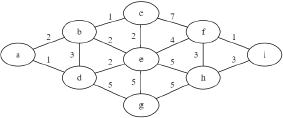
\includegraphics[height=0.3\textheight]{a01a_graph}
        \label{fig:a01_graph}
    \end{figure}

    \section{Lösung}

    \begin{minted}[
        frame=lines,
        framesep=2mm,
        baselinestretch=1.2,
        bgcolor=LightGray,
        linenos,
        breaklines
    ]{python}
def prim(G: nx.Graph, start_node: Any):

    if start_node not in G.nodes:
        raise ValueError(f'Start node {start_node} not in graph {G.nodes}')

    mst = nx.Graph()
    visited = {start_node}
    edges = [
        (data['weight'], start_node, to)
        for to, data in G[start_node].items()
    ]
    heapq.heapify(edges)

    while edges:
        weight, frm, to = heapq.heappop(edges)
        if to in visited:
            continue
        visited.add(to)
        mst.add_edge(frm, to, weight=weight)

        for to_next, data in G[to].items():
            if to_next not in visited:
                heapq.heappush(edges, (data['weight'], to, to_next))

    return mst
    \end{minted}

    \begin{figure}[htbp]
        \centering
        \begin{subfigure}[b]{0.45\textwidth}
            \centering
            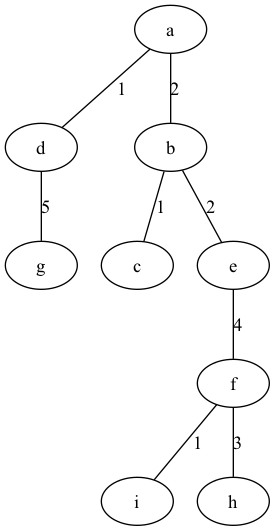
\includegraphics[width=\textwidth, height=6cm, keepaspectratio]{a01a_mst}
            \caption{Minimaler Spannbaum}
            \label{fig:a01_mst}
        \end{subfigure}
        \begin{subfigure}[b]{0.45\textwidth}
            \centering
            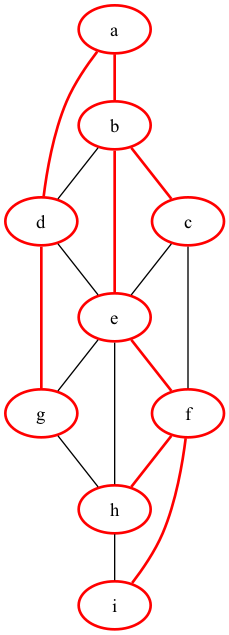
\includegraphics[width=\textwidth, height=6cm, keepaspectratio]{a01a_graph_highlighted}
            \caption{Minimaler Spannbaum auf dem Graphen}
            \label{fig:a01_graph_highlighted}
        \end{subfigure}
        \caption{Gegenüberstellung der Spannbäume}
        \label{fig:a01_comparison}
    \end{figure}

    Die Kosten des Spannbaumes sind 19.

    \newpage

    \chapter{Spannbaum Kruskal}
    \label{ch:sbkruskal}
    Für den Graphen aus \hyperref[fig:a01_graph]{Beispiel~1} suchen Sie einen minimalen Spannbaum mit dem Algorithmus von
    Kruskal und stellen Sie diesen dar. Unterscheidet sich dieser vom Spannbaum in Beispiel 1?

    \section{Lösung}

    \begin{minted}[
        frame=lines,
        framesep=2mm,
        baselinestretch=1.2,
        bgcolor=LightGray,
        linenos,
        breaklines
    ]{python}
def kruskal(G: nx.Graph):
    mst = nx.Graph()
    sorted_edges = sorted(G.edges(data=True), key=lambda x: x[2]['weight'])
    parent = {}
    rank = {}

    def find(node):
        if parent[node] != node:
            parent[node] = find(parent[node])
        return parent[node]

    def union(node1, node2):
        root1 = find(node1)
        root2 = find(node2)
        if root1 != root2:
            if rank[root1] > rank[root2]:
                parent[root2] = root1
            else:
                parent[root1] = root2
                if rank[root1] == rank[root2]:
                    rank[root2] += 1

    for node in G.nodes():
        parent[node] = node
        rank[node] = 0

    for edge in sorted_edges:
        weight, frm, to = edge[2]['weight'], edge[0], edge[1]
        if find(frm) != find(to):
            union(frm, to)
            mst.add_edge(frm, to, weight=weight)

    return mst
    \end{minted}

    \begin{figure}[htbp]
        \centering
        \begin{subfigure}[b]{0.45\textwidth}
            \centering
            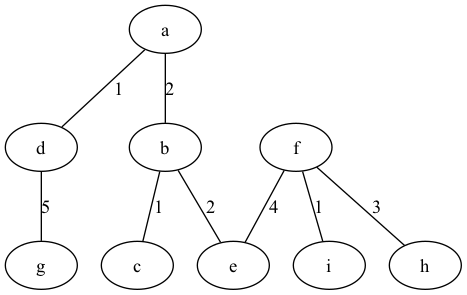
\includegraphics[width=\textwidth, height=6cm, keepaspectratio]{a02a_mst}
            \caption{Minimaler Spannbaum}
            \label{fig:a02_mst}
        \end{subfigure}
        \begin{subfigure}[b]{0.45\textwidth}
            \centering
            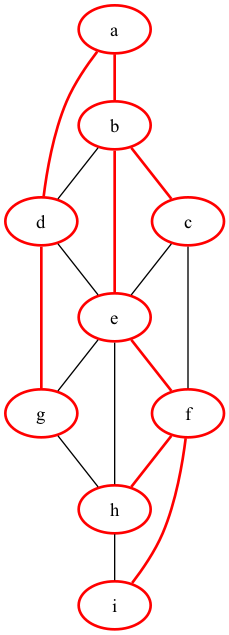
\includegraphics[width=\textwidth, height=6cm, keepaspectratio]{a02a_graph_highlighted}
            \caption{Minimaler Spannbaum auf dem Graphen}
            \label{fig:a02_graph_highlighted}
        \end{subfigure}
        \caption{Gegenüberstellung der Spannbäume}
        \label{fig:a02_comparison}
    \end{figure}

    Die Kosten des Spannbaumes sind 19.

    \newpage

    \chapter{Minimale Spannbäume}
    \label{ch:minSb}
    \begin{enumerate}
        \item Suchen Sie alle minimalen Spannbäume (MST) in folgendem Graph.
        \item Welche Kosten weisen diese auf?
        \item Stellen Sie die unterschiedlichen MST dar!

        \begin{figure}[H]
            \centering
            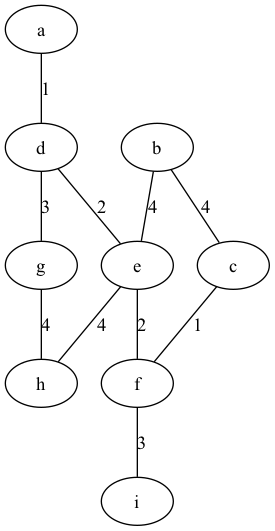
\includegraphics[height=0.3\textheight]{a03a_graph}
            \label{fig:a03_graph}
        \end{figure}

        \item Gegeben ein minimaler Spannbaum $T$ von einem Graph $G$. \hfill
        Wie kann geprüft werden ob es weitere MST in $G$ gibt oder ob $T$ einzigartig ist?
    \end{enumerate}

    \section{Lösung}




    \newpage

    \chapter{Die MST-Heuristik für das TSP}
    \label{ch:mstHeuristicTSP}
    Eine bewährte Methode gute (wenn auch nicht optimale) Rundreisen zu finden, fußt auf minimalen Spannbäumen.
    Bilden Sie für den Graphen $G$ (siehe Code unten), eine solche heuristische Rundreise mittels MST-Heuristik.
    Ermitteln Sie dazu:

    \begin{enumerate}[a)]
        \item einen minimalen Spannbaum MST
        \item einen gerichteten Graphen $G2$ bei dem jede Verbindung in MST durch eine Hin- und
        eine Zurückkante dargestellt wird
        \item einen Eulerkreis $k$ in $G2$ der in Linz beginnt und endet
        \item einen Hamiltonkreis $r$ in $G$ in dem Sie $k$ folgen und bereits besuchte Knoten
        überspringen
    \end{enumerate}

    \begin{minted}[
        frame=lines,
        framesep=2mm,
        baselinestretch=1.2,
        bgcolor=LightGray,
        linenos,
        breaklines
    ]{python}
G = nx.Graph()
G.add_weighted_edges_from([
    ("Wien", "Linz",184.4),
    ("Wien", "Hagenberg",180),
    ("Wien", "Graz",200.1),
    ("Wien", "Salzburg",295),
    ("Wien", "Steyr",166),
    ("Wien", "Wels",197),
    ("Linz", "Hagenberg",23),
    ("Linz", "Graz",220.9),
    ("Linz", "Salzburg",132.5),
    ("Linz", "Wels",132.5),
    ("Linz", "Steyr",132.5),
    ("Salzburg", "Steyr",134),
    ("Salzburg", "Graz",296),
    ("Salzburg", "Wels",108),
    ("Salzburg", "Hagenberg",155),
    ("Graz", "Steyr",191),
    ("Graz", "Wels",196),
    ("Graz", "Hagenberg",243),
    ("Wels", "Steyr",45.2),
    ("Wels", "Hagenberg",57.2),
    ("Steyr", "Hagenberg",43.6)
])
    \end{minted}

    \section{Lösung}

    \begin{enumerate}[a)]
        \item einen \hyperref[fig:a04_mst_and_highlight]{minimalen Spannbaum MST}
        \begin{figure}[htbp]
            \centering
            \begin{subfigure}[b]{0.3\textwidth}
                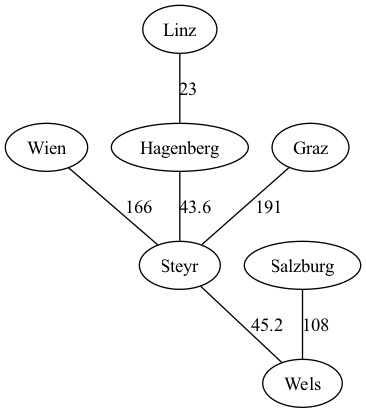
\includegraphics[height=6cm]{a04a_mst}
                \label{fig:a04_mst}
            \end{subfigure}
            \begin{subfigure}[b]{0.3\textwidth}
                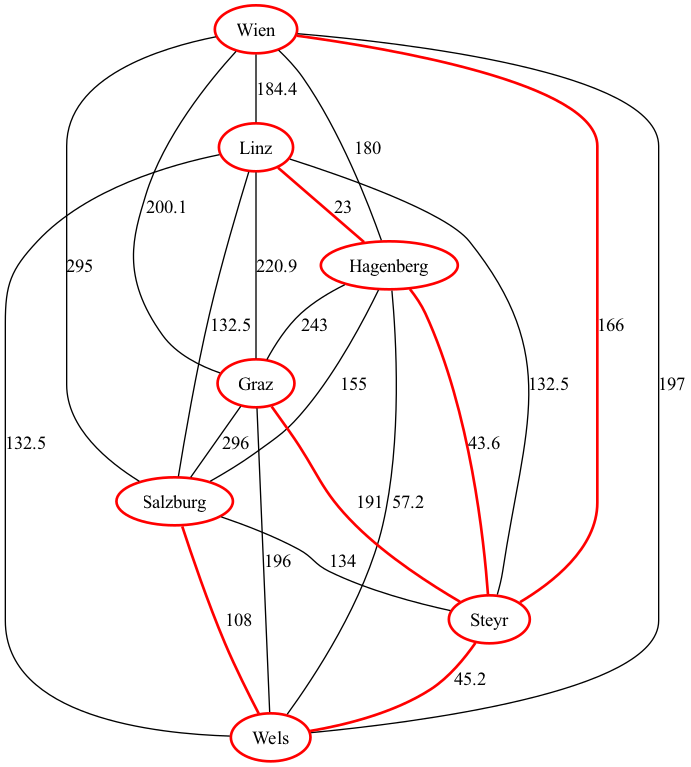
\includegraphics[height=6cm]{a04a_graph_highlighted}
                \label{fig:a04_graph_highlighted}
            \end{subfigure}
            \caption{Minimaler Spannbaum}
            \label{fig:a04_mst_and_highlight}
        \end{figure}

        \item einen \hyperref[fig:a04_g2]{gerichteten Graphen $G2$} bei dem jede Verbindung in MST durch eine Hin- und
        eine Zurückkante dargestellt wird
        \begin{figure}[htbp]
            \centering
            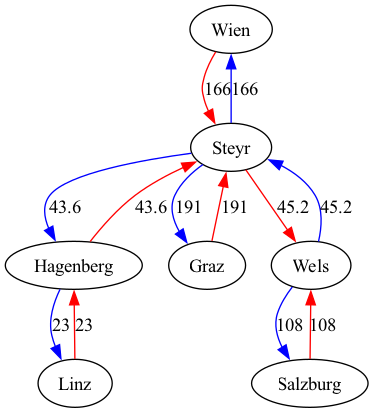
\includegraphics[height=6cm]{a04a_g2}
            \caption{Gerichter Graph G2}
            \label{fig:a04_g2}
        \end{figure}

        \item einen \hyperref[fig:a04_euler]{Eulerkreis $k$ in $G2$} der in Linz beginnt und endet
        \begin{figure}[htbp]
            \centering
            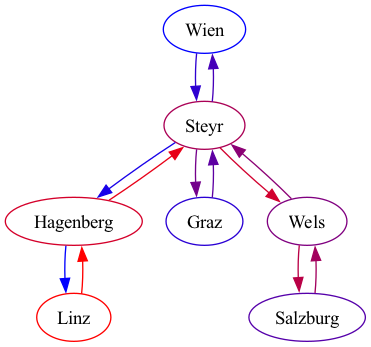
\includegraphics[height=6cm]{a04a_euler}
            \caption{Eulerkreis in gerichter Graph G2 von Linz nach Linz}
            \label{fig:a04_euler}
        \end{figure}

        \item einen \hyperref[fig:a04_hamilton]{Hamiltonkreis $r$ in $G$} in dem Sie $k$ folgen und bereits besuchte Knoten
        überspringen
        \begin{figure}[htbp]
            \centering
            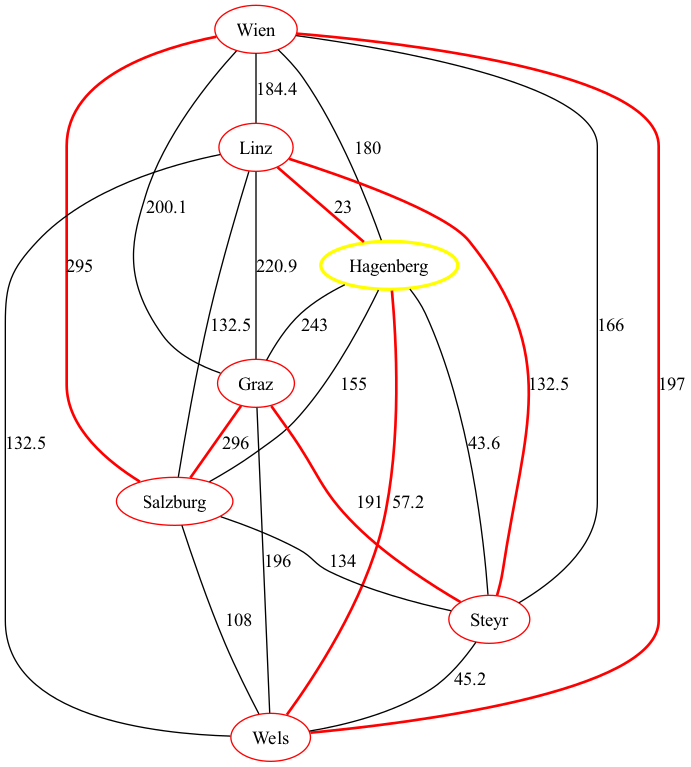
\includegraphics[height=6cm]{a04a_hamilton_highlighted}
            \caption{Hamilton Kreis im Graphen $G$}
            \label{fig:a04_hamilton}
        \end{figure}

    \end{enumerate}

    \newpage

    \chapter{Minimale Spannbäume in gerichteten Graphen}
    \label{ch:minSbDiGraph}
    Recherchieren Sie nach minimalen Spannbäumen für gerichtete Graphen.
    Sind die Algorithmen von Prim und Kruskal für gerichtete Graphen anwendbar?
    Warum (nicht)?

    \section{Lösung}

    Sowohl Prim's als auch Kruskal's Algorithmus kann nicht mit gerichteten Graphen umgehen.
    Es gibt jedoch den \href{https://www.wikiwand.com/en/Edmonds%27_algorithm}{Algorithmus von Edmond's bzw. Chu–Liu/Edmond's} welcher das Minimale Spannbaum Problem für gerichtete Graphen Löst.

    \subsection{Prombleme mit Prim's Algorithmus in Gerichteten Graphen}
    Prims Algorithmus basiert auf der Annahme, dass alle Knoten von einem Knoten aus erreichbar sind.
    In einem gerichteten Graphen $G$ ist dies nicht immer der Fall, z.B. wenn ein Knoten und eingehende Kanten hat.

    \begin{figure}[htbp]
        \centering
        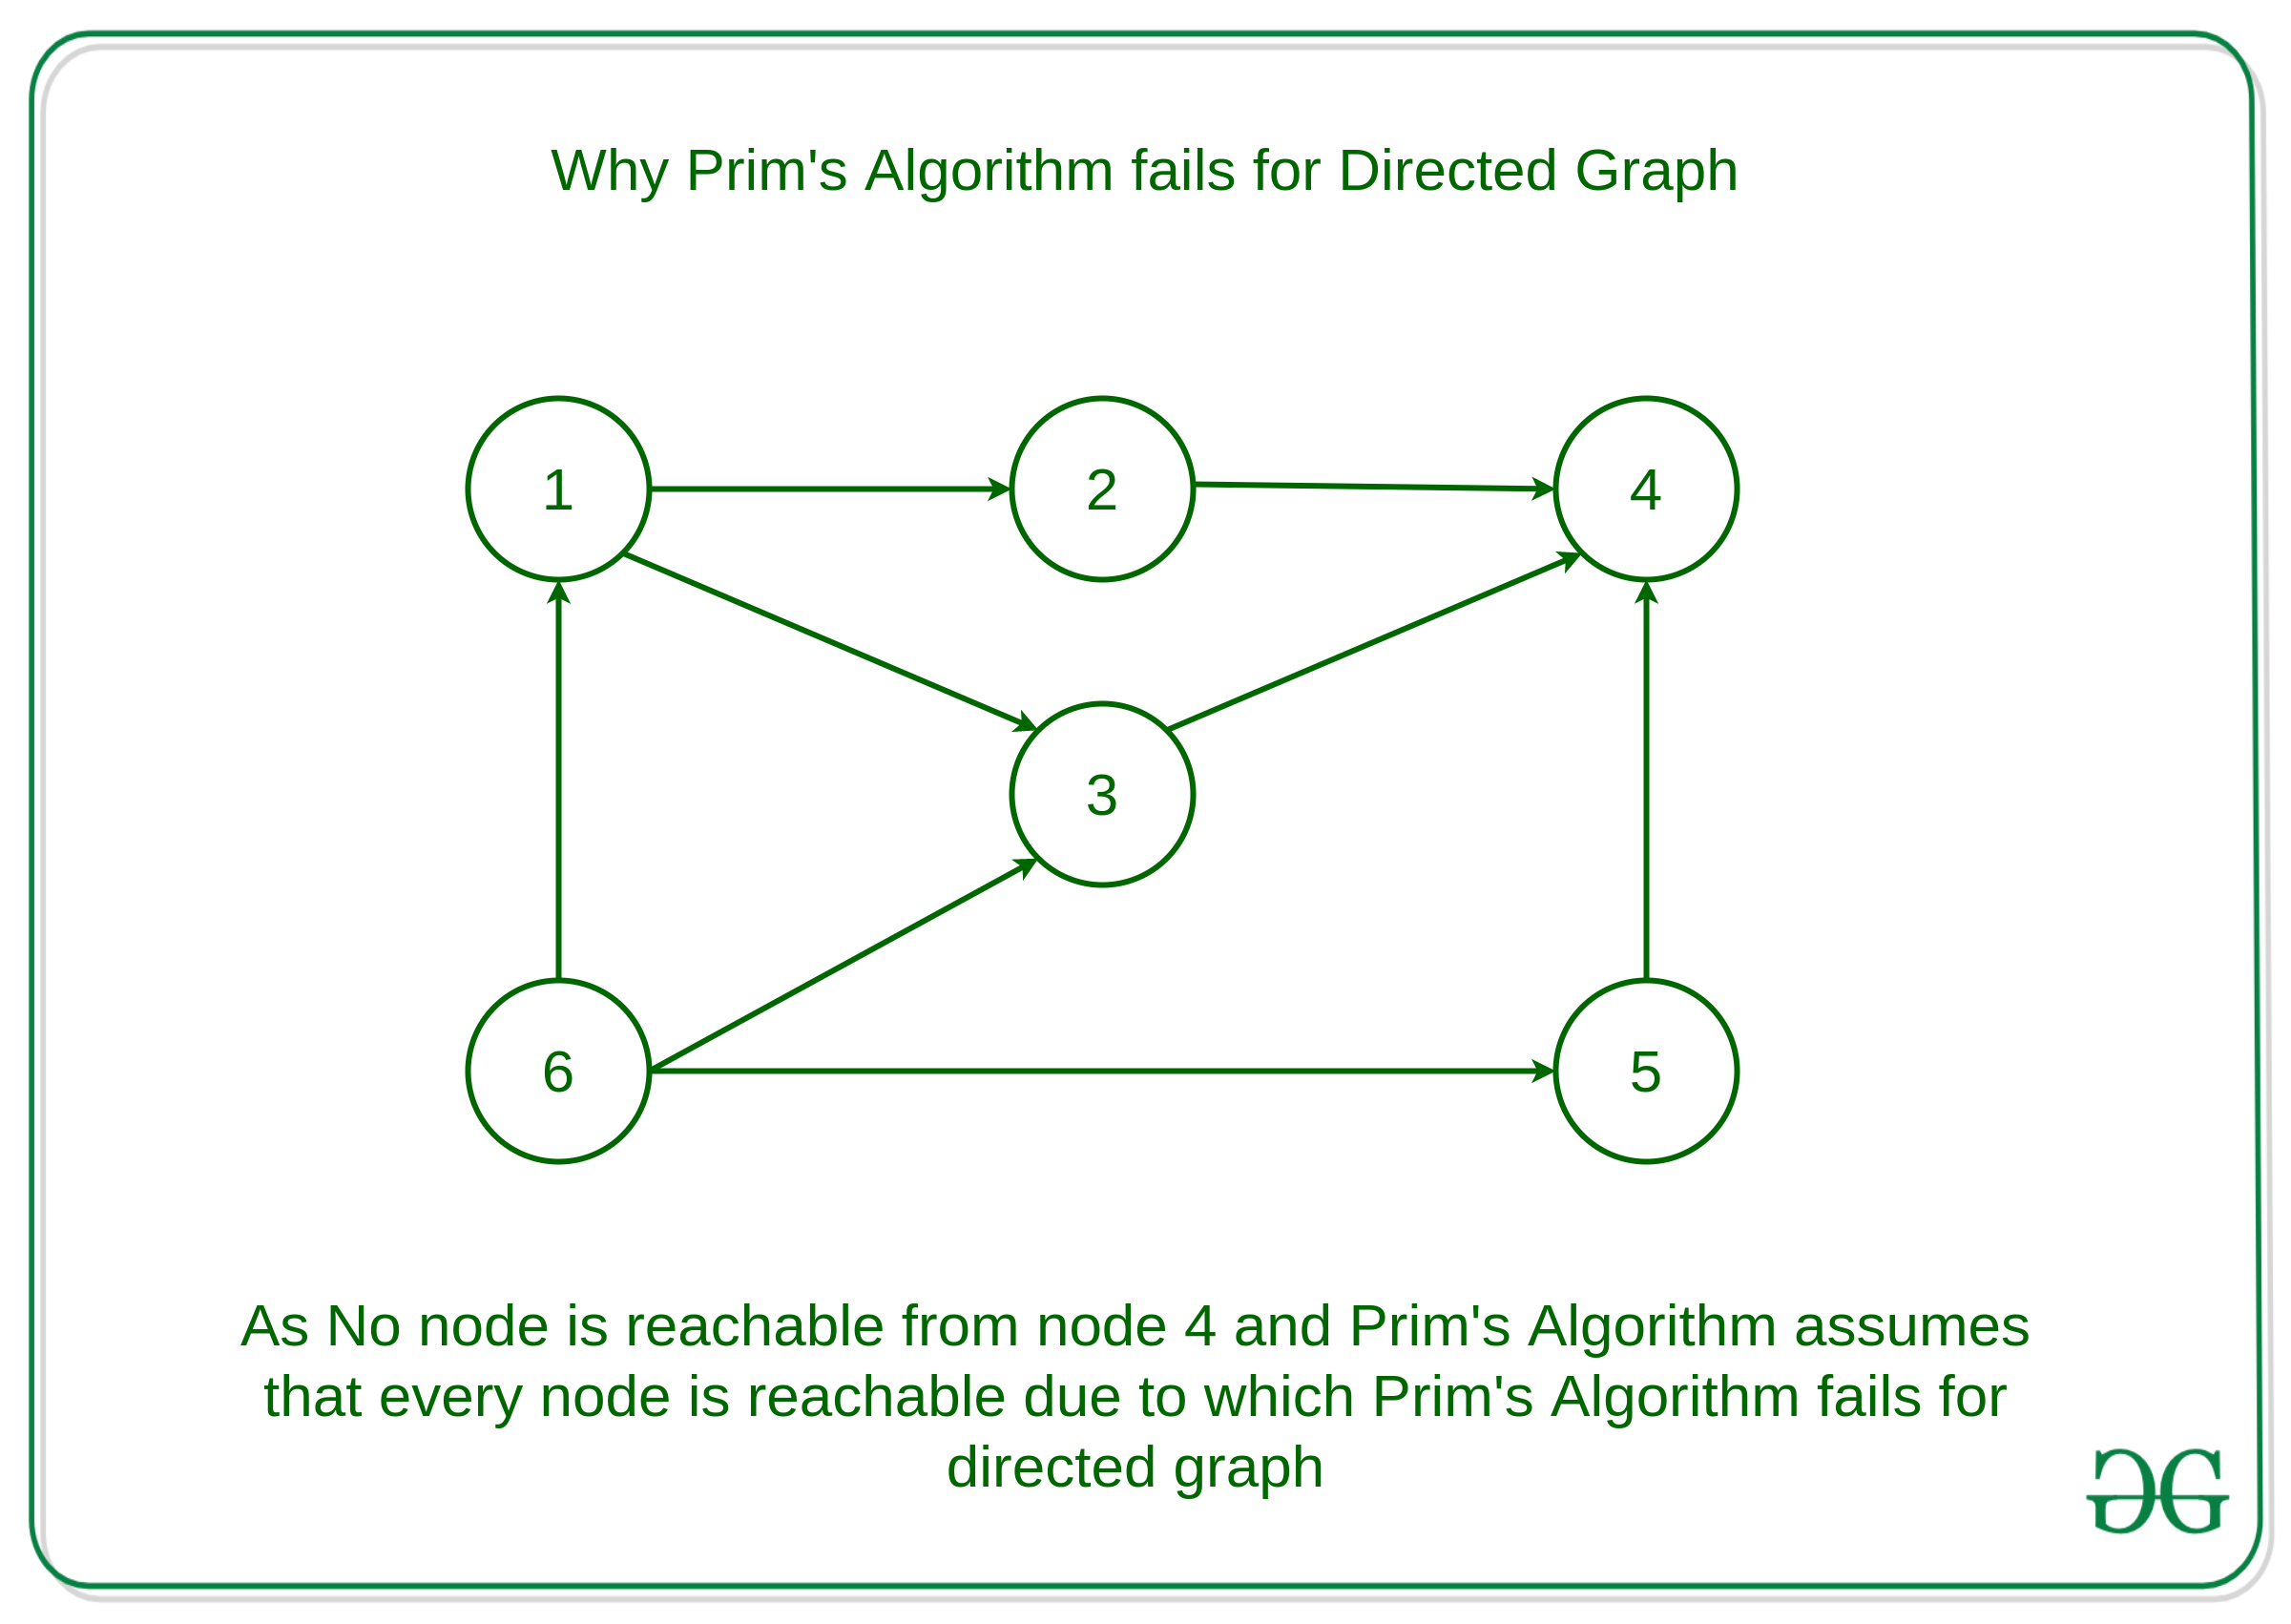
\includegraphics[height=6cm]{a05a_prims_issue}
        \caption{Problem bei Prim's Algorithmus. Quelle: \href{https://www.geeksforgeeks.org/why-prims-and-kruskals-mst-algorithm-fails-for-directed-graph/}{geeksforgeeks.org}}
        \label{fig:a05_prim}
    \end{figure}

    \subsection{Prombleme mit Kruskals's Algorithmus in Gerichteten Graphen}
    Kruskals Algorithmus überprüft in jeder Iteration, ob die zuletzt hinzugefügte Kante einen Kreis mit dem bestehenden MST bildet.
    Jedoch kann es vorkommen, dass Kruskals Algorithmus einen Kreis in einem gerichteten Graphen nicht finden kann,
    oder umgekehrt, einen Kreis in einem gerichtetem Graphen findet, in welchem es keinem gibt.
    Dies liegt an der \texttt{Union-Find} Methode welch standardmäßig verwendet wird.

    \begin{figure}[htbp]
        \centering
        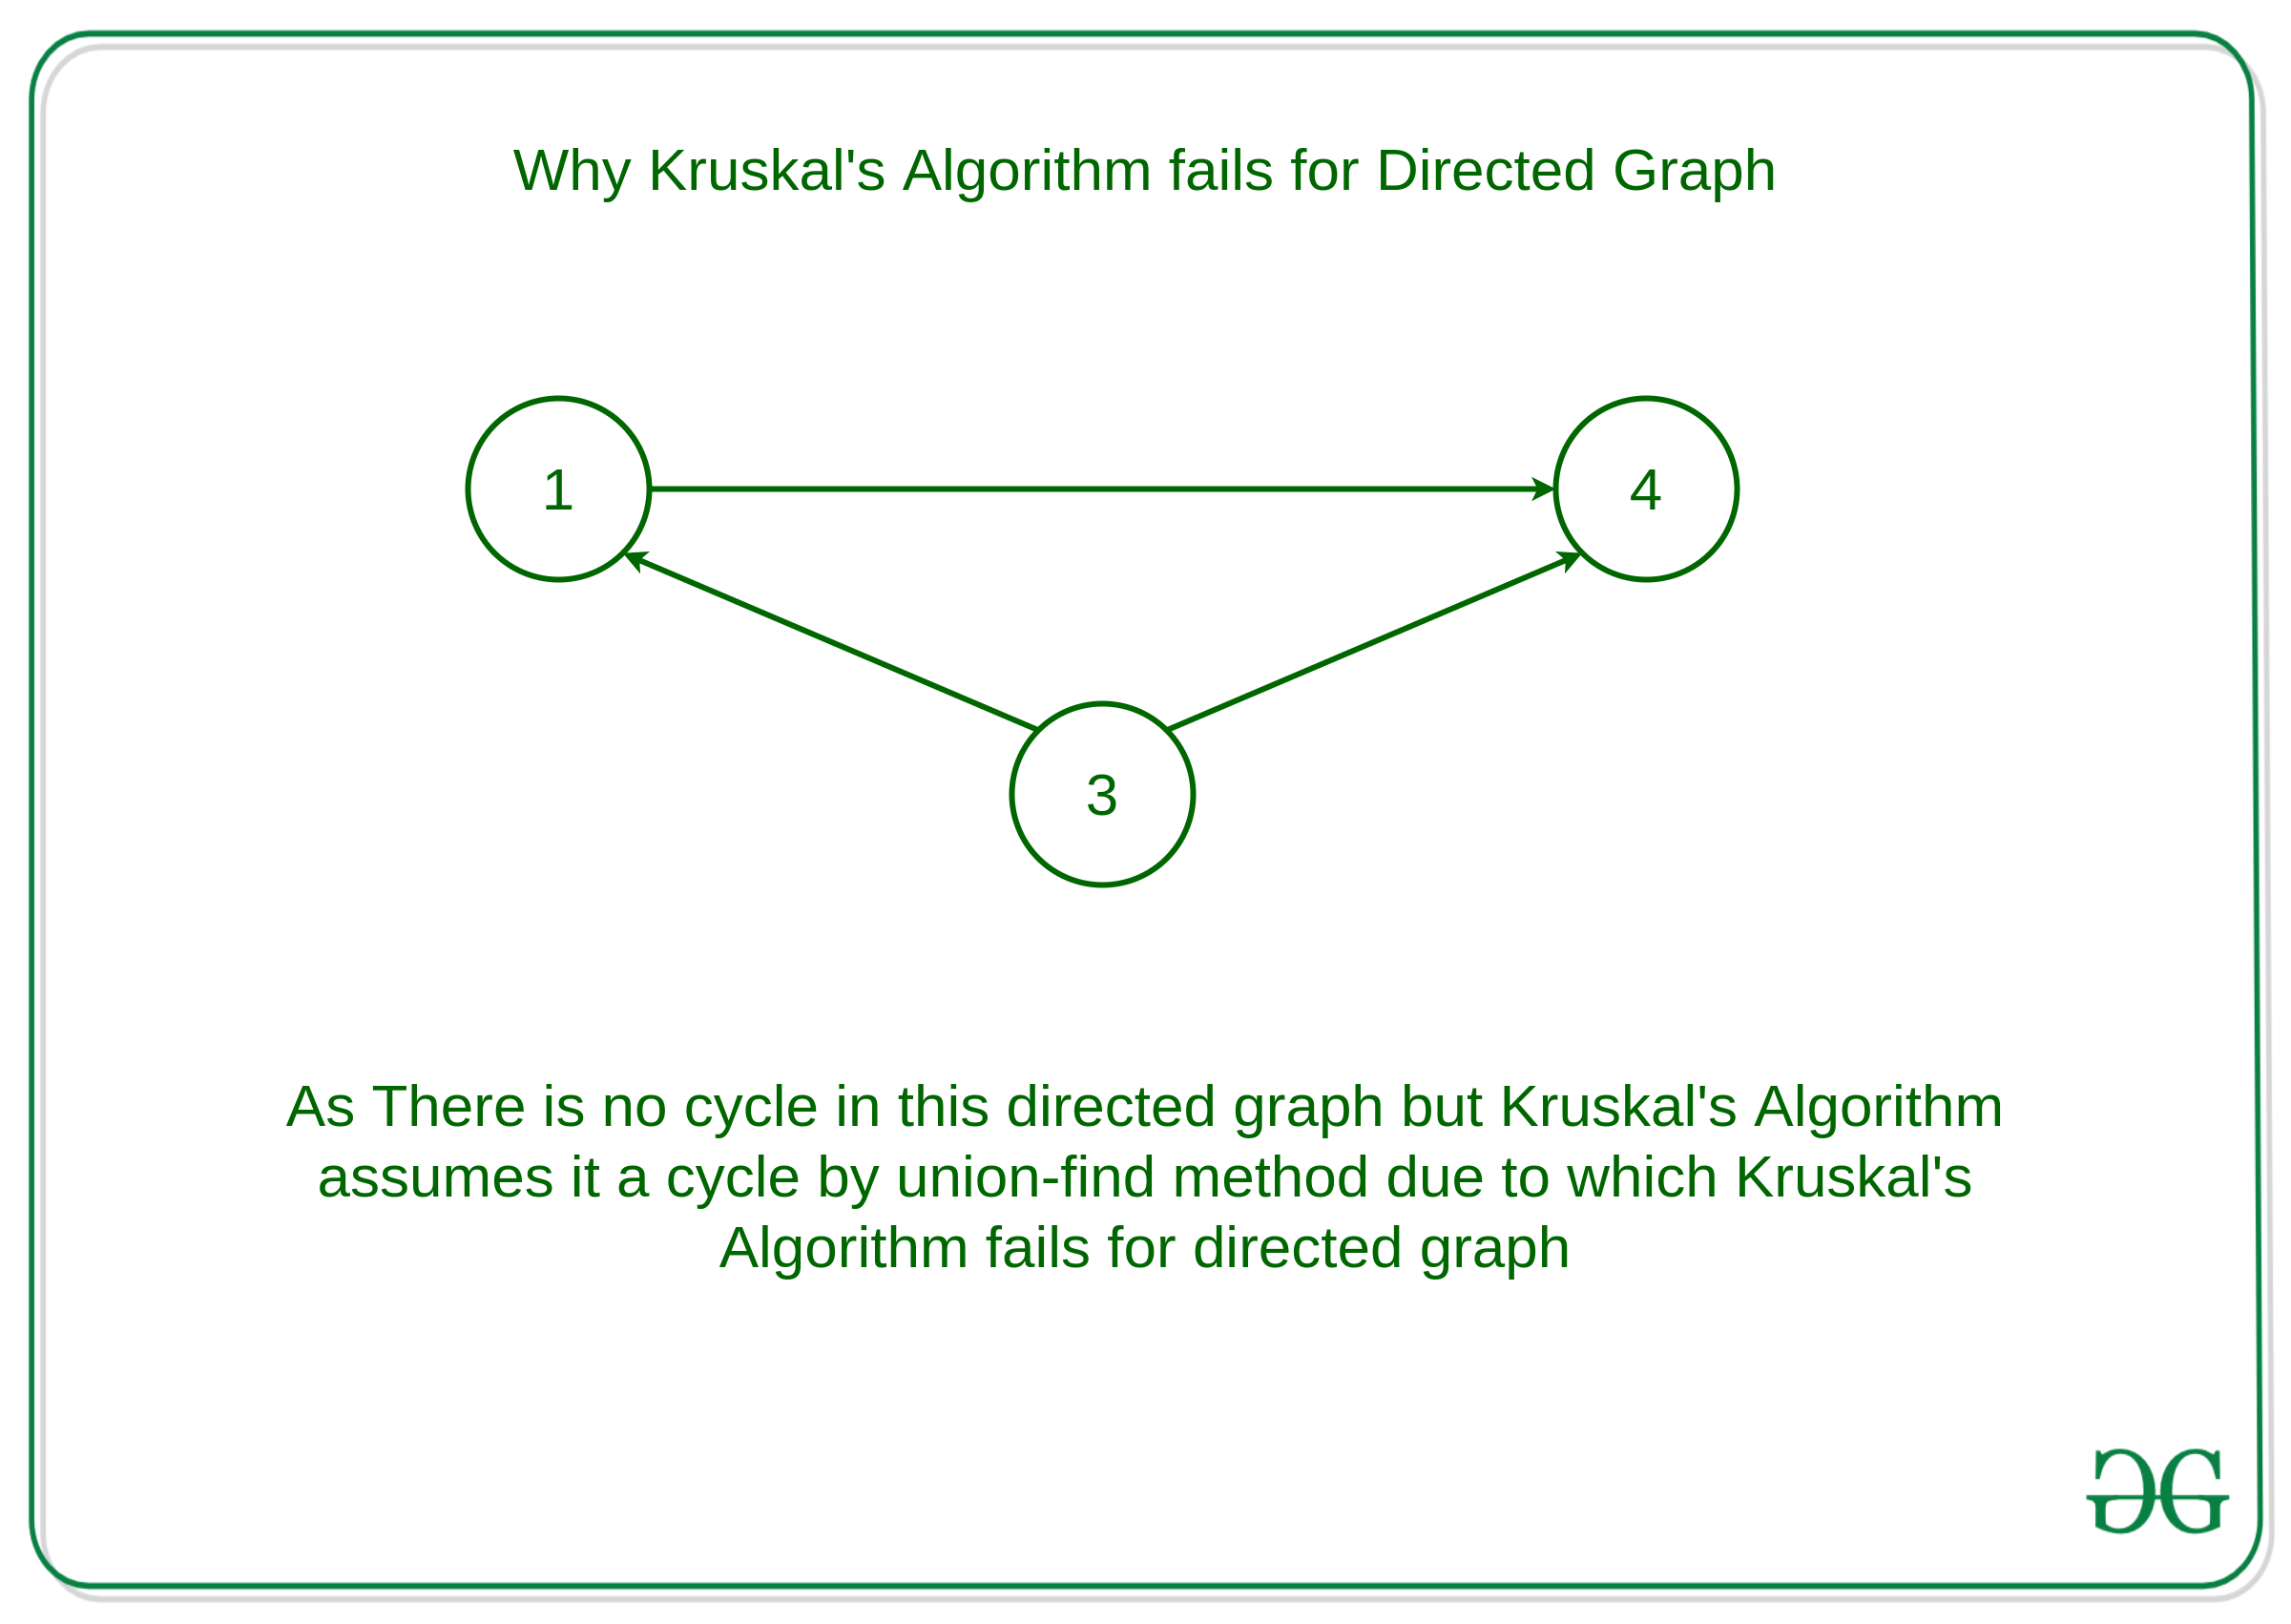
\includegraphics[height=6cm]{a05a_kruskals_issue}
        \caption{Problem bei Kruskals's Algorithmus. Quelle: \href{https://www.geeksforgeeks.org/why-prims-and-kruskals-mst-algorithm-fails-for-directed-graph/}{geeksforgeeks.org}}
        \label{fig:a05_kruskal}
    \end{figure}
    \newpage

    \chapter{PageRank}
    \label{ch:pageRank}
    Bestimmen Sie die Matrizen $\widetilde{A}$, $\widetilde{A}$ und $M$ für den Dämpfungsfaktor $d = 0.75$ und stellen Sie diese dar.
    Berechnen Sie den PageRank, geben Sie den Vektor $R$ nach den ersten $3$ Iterationen aus dem Potenzverfahren an (Initialwert $R_0$, $R_1$, $R_2$, $R_3$) wobei die Zahl im Index für die Iteration steht.
    Was bedeutet der PageRank?

    \begin{figure}[H]
        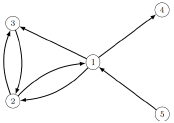
\includegraphics[width=0.3\textwidth]{a06a_graph}
        \label{fig:a06_graph}
    \end{figure}

    \section{Lösung}

    \begin{minted}[
        frame=lines,
        framesep=2mm,
        baselinestretch=1.2,
        bgcolor=LightGray,
        linenos,
        breaklines
    ]{python}
def create_transition_matrix(G, d=0.75):
    N = len(G.nodes)
    A = nx.adjacency_matrix(G, nodelist=sorted(G.nodes)).todense()
    A = np.array(A, dtype=float)
    out_degree = np.sum(A, axis=1)

    # Avoid division by zero by setting 1 where out_degree is 0
    out_degree[out_degree == 0] = 1
    M = A / out_degree

    # Calculate the Google matrix with damping factor
    G_matrix = d * M + (1 - d) / N * np.ones((N, N))

    return G_matrix, M

def pagerank(G, d=0.75, iterations=3):
    N = len(G.nodes)
    G_matrix, M = create_transition_matrix(G, d)

    # Initial vector R_0
    R = np.ones(N) / N

    R_list = [R]
    for _ in range(iterations):
        R = np.dot(G_matrix, R)
        R_list.append(R)

    return R_list, G_matrix, M
    \end{minted}

    \begin{minted}[
        frame=lines,
        framesep=2mm,
        baselinestretch=1.2,
        bgcolor=LightGray,
        linenos,
        breaklines
    ]{text}
R_0 = [0.2 0.2 0.2 0.2 0.2]
R_1 = [0.425 0.25  0.05  0.05  0.1  ]
R_2 = [0.2125  0.1875  0.04375 0.04375 0.15   ]
R_3 = [0.1678125 0.1178125 0.031875  0.031875  0.085    ]

Google Matrix G (with damping factor d=0.75):
 [
 [0.05  0.425 0.8   0.8   0.05 ]
 [0.3   0.05  0.8   0.05  0.05 ]
 [0.05  0.05  0.05  0.05  0.05 ]
 [0.05  0.05  0.05  0.05  0.05 ]
 [0.3   0.05  0.05  0.05  0.05 ]
 ]

Transition Matrix M:
 [
 [0.         0.5        1.         1.         0.        ]
 [0.33333333 0.         1.         0.         0.        ]
 [0.         0.         0.         0.         0.        ]
 [0.         0.         0.         0.         0.        ]
 [0.33333333 0.         0.         0.         0.        ]
 ]
    \end{minted}


    \newpage

    \chapter[Page Rank als Simulation]{Page~Rank als Simulation}
    \label{ch:pageRankSim}

    \begin{wrapfigure}{r}{0.32\textwidth}
        \centering
        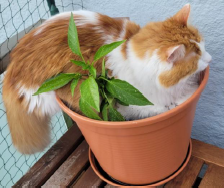
\includegraphics[width=0.3\textwidth]{a07a_cat}
        \label{fig:a06_cat}
    \end{wrapfigure}

    Aurora hat in der Küche zu viel Katzengras erwischt und ist dementsprechend berauscht.
    Sie können die Katze im untenstehenden Routinggraf der Wohnung Ihres Übungsleiters als „Random cat-agent“ annehmen,
    der in jedem Zeitschritt zufällige Kanten wählt (auch zurück).
    Wenn die Katze eines der drei Katzenbetten erreicht, legt sie sich dort schlafen (Katzenbetten sind Senken).
    In welchem Bett wird Sie die Katze mit welcher Wahrscheinlichkeit nach einer sehr großen Anzahl an Zeitschritten auffinden?
    Nach wie vielen Iterationen beträgt die Gesamtwahrscheinlichkeit, dass die Katze irgendein Bett erreicht, hat über 30\%?

    \begin{figure}[h]
        \centering
        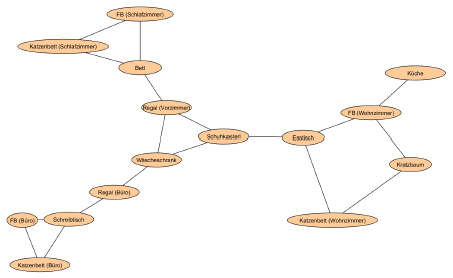
\includegraphics[width=0.8\textwidth]{a07a_graph}
        \label{fig:a07_graph}
    \end{figure}

    \section{Lösung}

    \begin{figure}[htbp]
        \centering
        \begin{subfigure}[b]{0.49\textwidth}
            \begin{minted}[
            frame=lines,
            framesep=2mm,
            baselinestretch=1.2,
            bgcolor=LightGray,
            linenos,
            breaklines
            ]{text}
Probability to stay in sink i.e. for Aurora to get stick in a bed:
Katzenbett (Schlafzimmer): 1.01%
Katzenbett (Büro): 1.03%
Katzenbett (Wohnzimmer): 0.94%
        \end{minted}
            \label{fig:a07_output}
        \end{subfigure}
        \begin{subfigure}[b]{0.49\textwidth}
            
\includegraphics[height=8cm]{a07a_probability}
            \label{fig:a07_plot}
        \end{subfigure}
        \label{fig:a07_solution}
    \end{figure}


    \newpage

    \chapter{Legal}
    \label{ch:legal}
    Die Ausarbeitung der Aufgabe wurde durch:

    \begin{itemize}
        \item \texttt{OpenAI - GPT-4.5 Turbo}
        \item \texttt{OpenAI - GPT-4.5 Vision}
        \item \texttt{OpenAI - GPT-4o}
        \item \texttt{Anthropic -- Claude 3 Opus}
    \end{itemize}

    mit mehreren unterschiedlichen Prompts und Custom Instructions unterstützt.

\end{document}